Nous avons choisi le projet tuteuré suivant : rendu temps réel de scènes complexes et interaction dans un navigateur.
Nous avons pour objectif de générer aléatoirement un monde "Lego" virtuel et de pouvoir intéragir avec. En fonction de
l'altitude, les textures changerons afin de représenter de l'eau, des prairies, et des montagnes. Nous avons utilisé
l'algorithme de génération du bruit de Perlin, et à terme nous implémenterons la version améliorée : la version avec les simplex.
Après avoir étudier les différentes technologie présente sur le net, nous avons choisi l'API three.JS, car elle est très bien
documentée. Cette API est écrite en JavaScript.

\begin{center}
	\null\vspace{0.25cm}
	
\includegraphics[height=3cm]{images/logo_threeJS.png}\\
	\textit{Logo de l'API three.JS}\\
\end{center}

Le tout sera couplé avec une page HTML, et une feuille de style. L'HTML sera le liant entre la feuille de style CSS, et le script en JavaScript, que va éxécuté le client web pour afficher notre monde virtuel.
Voici un schéma montrant l'ensemble des technologies utilisées :

\begin{center}
	\null\vspace{0.25cm}
	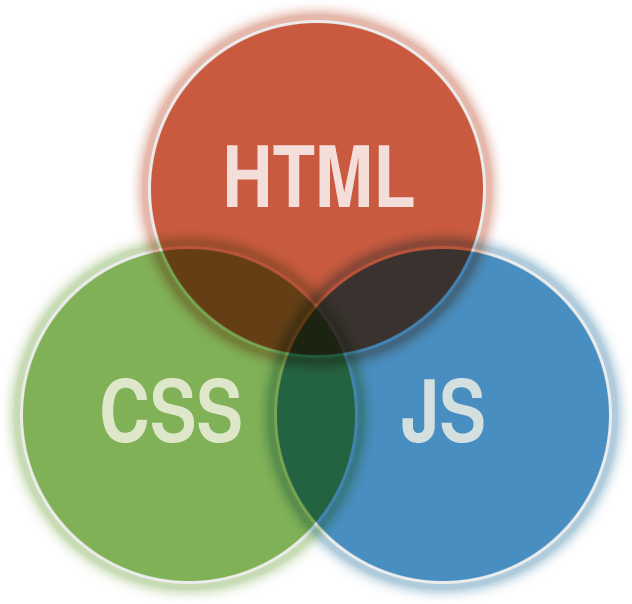
\includegraphics[height=3cm]{images/HTML_CSS_JS.png}\\
	\textit{Schéma des technologies utilisées}\\
\end{center}

